\documentclass[12pt]{article}

\usepackage[T1]{fontenc}
\usepackage[utf8]{inputenc}
\usepackage{lmodern}
\usepackage[margin=1.1in]{geometry}
\usepackage{amsmath,amssymb}
\usepackage{booktabs}
\usepackage{graphicx}
\usepackage{caption}
\usepackage{setspace}
\usepackage[round,authoryear]{natbib}
\usepackage[hidelinks]{hyperref}
\usepackage{microtype}

\captionsetup{font=small,labelfont=bf,width=.95\textwidth}
\setlength{\parindent}{1.6em}
\onehalfspacing

\title{\textbf{Digital Mice: Inducing and Validating\\ Controlled Cognitive Deficits in Frontier\\ Language Models for Mechanism Design}}
\author{}
\date{\today}

\begin{document}
\maketitle

\begin{abstract}
\noindent Early-stage mechanism design is a phase-I science: the relevant
behavior is human cognition, so designers must run experiments on people
before they can learn which mechanisms are robust to bounded rationality. We
ask whether frontier reasoning models can serve as the economist's analogue of
the laboratory mouse---capable reasoners instructed into specific, controlled
cognitive deficits whose behavior can be studied before human subjects are
recruited. Using a canonical second-price sealed-bid auction (SPSB) and a
$3\times 3\times 3$ panel of \emph{digital mice} defined over three cognitive
axes (contingent reasoning, forward planning, belief reasoning), we establish
three facts. First, the deficits have \emph{construct validity}: repairing each
axis moves truthful bidding in the theory-predicted direction, monotonically
and with the predicted sign in all five pre-registered directional tests.
Second, the panel---augmented by a small set of targeted error strains---attains
\emph{calibration coverage}: it reproduces all five canonical SPSB human-mistake
classes (truthful, moderate underbidding, overbidding, extreme overbidding,
and near-zero bidding) at rates above their detection thresholds. Third, the
panel is \emph{discriminating}: in a first-price sealed-bid stress test the
reasoning strains track the risk-neutral Bayes--Nash benchmark ($b=\tfrac23 v$),
overbid relative to it at the rate documented for human subjects, and a strain
that overgeneralizes the second-price payment rule overbids above value and
loses money---a mechanistic account of a winner's-curse pathology. We also show
that augmenting the deficit instruction with a worked chain-of-thought
demonstration sharpens and stabilizes the induced behavior, and that at the
strain level four of five reserved deficits preserve their behavioral class
across base models. These results support the use of instructed-deficit language
models as a phase-I screening population for mechanism design.

\vspace{0.6em}
\noindent\textit{Keywords:} bounded rationality, mechanism design, second-price
auctions, large language models, construct validity.
\end{abstract}

\section{Introduction}

Medicine studies humans, but it does not begin with them. Much early drug
testing starts with mice, and some of those mice are deliberately engineered to
lack a specific protein, receptor, or channel. The deficit is not a nuisance;
it is the identification strategy. If a treatment succeeds or fails only when a
particular channel is removed, the experiment isolates a mechanism that is
entangled in an intact organism.

Economics has lacked this luxury. The behavior of interest in mechanism design
is human cognition---contingent reasoning, forward planning, belief formation,
and strategic sophistication---and these channels are bundled in real subjects.
A bidder who fails to bid truthfully in a strategy-proof auction may lack
contingent reasoning, may fail to plan forward, may hold incorrect beliefs
about rivals, or may simply misunderstand the rule. Natural and laboratory
experiments rarely deliver a population missing exactly one cognitive module,
so the empirical content of theories such as obvious strategy-proofness
\citep{li2017}, cursed equilibrium \citep{eysterrabin2005}, and level-$k$
reasoning \citep{crawfordiriberri2007} is hard to separate.

Large language models change the experimental object. The strongest current
reasoning models are, in simple games, often closer to a fully rational agent
than an ordinary subject: they follow long chains of reasoning and compute
through cases. That capability is precisely what makes them useful here. We
start from a capable reasoning substrate and instruct it to ``play dumb'' in a
controlled way---reason only myopically, enumerate only local contingencies,
ignore second-order beliefs---through explicit procedural constraints on its
deliberation, not through dependence on hidden quirks of one model. This yields
\emph{digital mice}: language-model agents with specific, engineered cognitive
deficits.

\paragraph{Research question.} Can a frontier reasoning model be instructed
into stable, separable bounded-rationality states that (i) produce the
behavioral signatures predicted by cognitive theory and (ii) span the
empirically documented space of human mistakes, in a canonical second-price
sealed-bid auction?

\paragraph{Contribution.} We answer both halves affirmatively for the SPSB
environment. Over a $3\times 3\times 3$ panel of $27$ strains ($810$
bidder-decisions), repairing each cognitive axis raises the truthful-bid rate
by $+0.23$ (contingent reasoning), $+0.14$ (forward planning), and $+0.05$
(belief reasoning); all five pre-registered directional hypotheses pass their
sign test. The panel, augmented by two targeted error strains, covers all five
canonical SPSB human-mistake classes at rates above threshold. Third, in a
first-price stress test the reasoning strains shade to the risk-neutral BNE
($b=\tfrac23 v$, median ratios $0.65$--$0.67$) and overbid relative to it at
$38\%$, while the second-price-overgeneralizer mouse bids above value and loses
money. Along the way we show that a worked chain-of-thought demonstration is a
stronger control than instruction alone---it drives the all-deficit strain's
truthful rate from $0.39$ to $0$ and the all-repaired strain's to a perfect $1.0$
while lowering bid dispersion---and that four of five reserved deficits keep their
behavioral class across base models. We are explicit about a boundary of the
construction: the clean procedural basis naturally produces truthful and
underbidding behavior but not overbidding, which we recover with a small number
of hand-specified heuristic strains. We treat the digital-mouse panel as phase-I
screening evidence, not as a prediction of human population shares.

\section{The Digital-Mouse Panel}

\subsection{Construction: a rational base plus a deficit instruction}

A digital mouse is a single prompt assembled from two layers. The first layer,
the \emph{rational base}, is identical across all strains and instructs the
model to play the auction as a long-run profit maximizer:

\begin{quote}\small\itshape
Your TOP PRIORITY is to place bids which maximize your profit in the long run.
Learn from the history of previous rounds in order to maximize your total
profit. Don't forget the values are redrawn independently each round.
\end{quote}

The second layer, \emph{defect induction}, appends a ``cognitive style'' block
containing exactly one paragraph per cognitive axis. Each paragraph constrains
the model's deliberation \emph{procedure}---not its objective---at one of three
levels. The intervention is therefore a reasoning-procedure control rather than
a payoff or preference change. Concretely, the contingent-reasoning axis ranges
from a level-0 paragraph that forbids reasoning about opponents to a level-2
paragraph that mandates a worst-case/dominance check:

\begin{quote}\small
\textbf{Contingent reasoning, level 0 (deficit).}\itshape{} Do NOT enumerate
possible bids by other bidders or compute best responses to specific opponent
moves. Choose your bid without conditioning on what others might do.
\end{quote}
\begin{quote}\small
\textbf{Contingent reasoning, level 2 (repaired).}\itshape{} For each possible
bid you could make, consider the worst-case outcome given the range of possible
opponent bids. Find the bid where even the worst-case outcome is acceptable. If
you deviated from this bid, could the worst case become worse?
\end{quote}

\noindent The forward-planning and belief-reasoning axes are constructed the
same way (from ``do not trace consequences'' to a multi-step decision tree, and
from ``do not model others'' to explicit second-order beliefs). A strain is thus
the rational base plus a triple $(c,f,b)\in\{0,1,2\}^3$ that selects one
paragraph for each axis. The all-off triple $(0,0,0)$ is the most deficient
mouse; the all-repaired triple $(2,2,2)$ is closest to the rational base.

\subsection{The $3\times 3\times 3$ grid}

Varying three axes at three levels each gives the $27$-strain panel of
Table~\ref{tab:panel}. A useful intuition: the rational base supplies the
\emph{goal} (maximize profit), and the cognitive-style block rations the
\emph{reasoning steps} the mouse is allowed to use to pursue it. A mouse told
not to enumerate opponents, not to trace payoffs, and not to model others must
fall back on a crude own-value heuristic; a mouse granted all three faculties
can in principle reconstruct the dominant strategy.

\begin{table}[t]
\centering
\caption{The $3\times 3\times 3$ digital-mouse panel. Each strain is one
combination of axis levels; the lowest level is the engineered deficit.}
\label{tab:panel}
\small
\setlength{\tabcolsep}{5pt}
\begin{tabular}{@{}llll@{}}
\toprule
Axis & Level 0 (deficit) & Level 1 & Level 2 (repaired) \\
\midrule
Contingent reasoning & no enumeration & enumerate cases & worst-case / dominance \\
Forward planning     & myopic & one-step lookahead & tree / multi-step \\
Belief reasoning     & no model of others & first-order beliefs & second-order beliefs \\
\bottomrule
\end{tabular}
\end{table}

\paragraph{Hardening the base (strict variant).} The base layer above makes
profit maximization the top priority, which leaves room for a very capable model
to ``see through'' a deficit and revert to the optimal strategy. For the
cross-model analysis of Section~6 we therefore also build a \emph{strict}
variant whose base layer inverts the priority---``follow the cognitive procedure
exactly\,\dots\ if the cognitive procedure conflicts with the profit-maximizing
strategy, the cognitive procedure wins''---and explicitly forbids invoking
dominant-strategy or Vickrey shortcuts. The strict variant is used only where
noted; all construct-validation and calibration results use the standard panel.

\section{Experimental Design and Methodology}

\paragraph{Environment.} The mechanism is a single-item second-price sealed-bid
auction with $N=3$ bidders. Private values are drawn independently and
uniformly on $[0,50]$; each bidder observes only its own value and submits one
sealed bid on a \$0.1 grid. Under standard preferences truthful bidding is a
weakly dominant strategy, which makes truthfulness a clean construct-validity
target: a more capable mouse should bid closer to its value.

\paragraph{Strains and runs.} We instantiate all $27$ basis strains with the
same base model (\texttt{gpt-5.4-mini}, temperature $0.5$) and collect $30$
bidder-decisions per strain ($810$ in total). Because the clean procedural
basis does not naturally generate \emph{overbidding}, we additionally author a
small set of targeted \emph{error mice}---heuristic strains designed to express
one documented mistake each (e.g.\ a ``second-price overgeneralizer'' that
treats bidding above value as safe because the winner pays the runner-up bid,
and a ``payment panic'' strain that bids near zero). Seven error strains are
specified; two had completed runs at the time of this analysis and feed the
calibration scorecard below.

\paragraph{Behavioral classes.} For each bidder-decision we record the bid, the
value, and the deviation $b-v$. We define a truthful bid as $|b-v|\le 0.05$,
moderate underbidding as $b<v-0.05$ (excluding near-zero bids), overbidding as
$b>v+0.05$, extreme overbidding as $b-v\ge 5$, and near-zero bidding as
$b\le 0.1$ with $v>5$. These thresholds operationalize the five canonical SPSB
mistake classes used in the calibration step.

\subsection{Outcome variables and the robustness objective}
\label{sec:fitness}

We now define the panel-based objective used to score mechanisms in Section~6.
Fix a mechanism and a persona panel $\mathcal{P}=\{p_1,\dots,p_M\}$, and run
$R$ independent auctions per persona. Index the resulting completed auctions by
$a\in\mathcal{A}$, with $\mathcal{A}_p$ the subset run under persona $p$. Each
auction has $N=3$ bidders with private values $v_{a,i}$ and elicited bids
$b_{a,i}$; the winner is $i^\star(a)=\arg\max_i b_{a,i}$ and the mechanism's
pricing rule sets the payment $\rho(a)$ (the second-highest bid under SPSB, the
own bid under all-pay, and so on). Let $A_{\text{att}}$ be the number of
\emph{attempted} auctions and $F$ the number that fail to parse or violate the
response format, so the failure rate is $\phi = F/A_{\text{att}}$.

\paragraph{Per-auction quantities.} Write $v^{\max}_a=\max_i v_{a,i}$. We use
allocative efficiency, a bid-shading dispersion, and realized winner surplus:
\begin{equation}
\mathrm{eff}(a)=\frac{v_{a,i^\star(a)}}{v^{\max}_a},
\qquad
s(a)=\operatorname{std}_{\,i:\,v_{a,i}>0}\!\left(\frac{b_{a,i}}{v_{a,i}}\right),
\qquad
\pi(a)=v_{a,i^\star(a)}-\rho(a).
\end{equation}

\paragraph{Panel aggregates.} With $A=|\mathcal{A}|$ and a value scale
$\bar v=\max_{a}v^{\max}_a$, define normalized revenue, mean efficiency, a
simplicity proxy, and normalized surplus variance:
\begin{equation}
\hat\rho=\frac{1}{A\,\bar v}\sum_{a}\rho(a),
\quad
\overline{\mathrm{eff}}=\frac1A\sum_{a}\mathrm{eff}(a),
\quad
\sigma=1-\frac1A\sum_{a}s(a),
\quad
\widehat{\mathrm{Var}}=\frac{\operatorname{Var}_a\!\big(\pi(a)\big)}{\bar v^{2}}.
\end{equation}
The simplicity proxy $\sigma$ is high when bidders converge on a common
bid/value ratio (an ``obvious'' mechanism) and low when their shading scatters.

\paragraph{Intended-action rate.} Each mechanism declares the action a correctly
reasoning bidder should take, $\tau\in\{\textsc{truthful},\textsc{shade},
\textsc{aggressive},\dots\}$, with tolerance $\epsilon=0.1$. For a scoreable
decision $(v,b)$ with $v>0$ define the match indicator
\begin{equation}
m_\tau(v,b)=
\begin{cases}
\mathbf{1}\!\left[\,|b-v|\le \epsilon\,\right] & \tau=\textsc{truthful},\\[2pt]
\mathbf{1}\!\left[\,\kappa < b < v-\epsilon\,\right] & \tau=\textsc{shade},\\[2pt]
\mathbf{1}\!\left[\,b+\epsilon \ge \alpha\, v\,\right] & \tau=\textsc{aggressive},
\end{cases}
\end{equation}
with floor $\kappa$ and aggressiveness threshold $\alpha=0.4$ by default. The
intended-action rate $\mu_\tau$ is the mean of $m_\tau$ over scoreable decisions;
targets labeled \textsc{unknown} or \textsc{mechanism-specific} are not scored
($\mu_\tau$ omitted).

\paragraph{Lower-tail (per-persona) statistics.} Let
$\overline{\mathrm{eff}}_p$, $\sigma_p$, and $\operatorname{Var}_p(\pi)$ be the
above computed within persona $p$. Robustness rewards good \emph{worst-case}
behavior across the panel, not just the average:
\begin{equation}
E_{\min}=\min_p \overline{\mathrm{eff}}_p,
\quad
E_{20}=Q_{0.2}\!\big(\{\overline{\mathrm{eff}}_p\}\big),
\quad
\Sigma_{\min}=\min_p \sigma_p,
\quad
\widehat V_{\max}=\frac{\max_p \operatorname{Var}_p(\pi)}{\bar v^{2}},
\end{equation}
where $Q_{0.2}$ is the $20$th percentile across personas.

\paragraph{Fitness.} The aggregate and robust fitness are weighted sums
\begin{align}
F_{\mathrm{agg}} &= w_1\hat\rho + w_2\overline{\mathrm{eff}} + w_3\mu_\tau
+ w_4\sigma - w_5\widehat{\mathrm{Var}} - w_6\phi,\\
F_{\mathrm{tail}} &= w_7 E_{\min} + w_8 E_{20} + w_9 \Sigma_{\min}
- w_{10}\widehat V_{\max},\\
F_{\mathrm{robust}} &= F_{\mathrm{agg}} + F_{\mathrm{tail}}.
\end{align}
Following the Stage-C calibration mapping, the default weights are
$(w_1,\dots,w_{10}) = (1,\,1,\,0.5,\,0.5,\,0.25,\,1,\,0.5,\,0.5,\,0.25,\,0.25)$,
grouping into domain performance $(w_1,w_2)$, intended action $(w_3)$, simplicity
$(w_4,w_9)$, regret $(w_5,w_{10})$, compliance $(w_6)$, and cognitive fragility
$(w_7,w_8)$. Section~6 reports $F_{\mathrm{robust}}$ and $\mu_\tau$; the
sign convention is that fragility, regret, and failure enter negatively, so a
mechanism scores well only if it is allocatively efficient, induces its intended
action, and does so \emph{uniformly} across the digital-mouse panel.

\section{Result 1: Construct Validity}

If the cognitive axes are genuine bounded-rationality controls rather than
arbitrary prompt artifacts, then repairing an axis should move behavior toward
the rational benchmark. Figure~\ref{fig:marginals} plots the truthful-bid rate
at each axis level, marginalizing over the other two axes. All three axes are
monotone or near-monotone in the repairing direction, and the contingent-reasoning
axis produces the largest swing.

\begin{figure}[t]
\centering
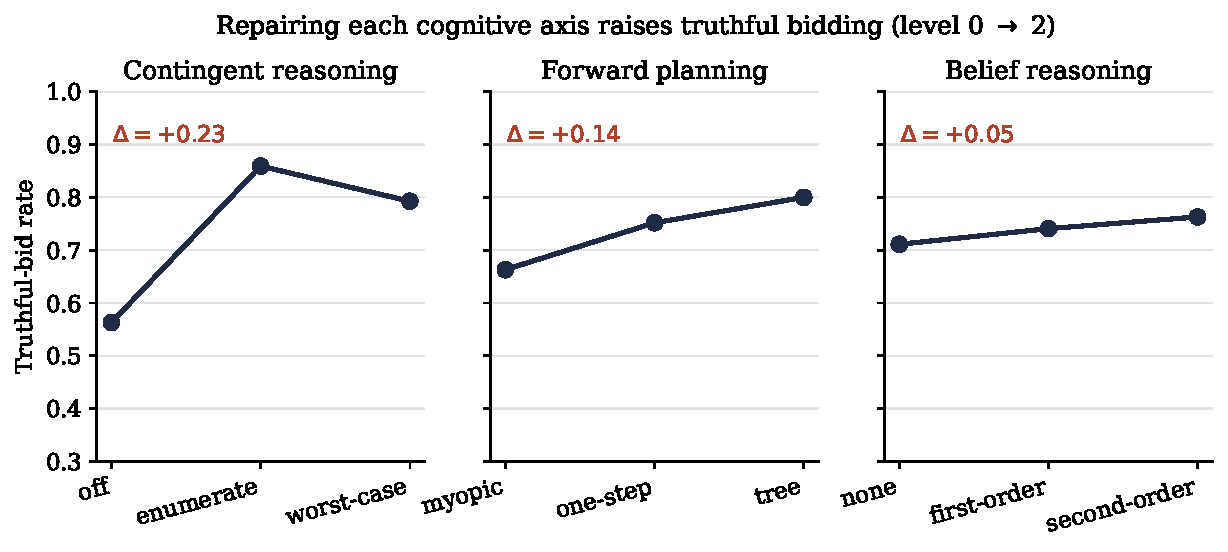
\includegraphics[width=\textwidth]{fig1.pdf}
\caption{Construct-validity marginals. Truthful-bid rate at levels 0/1/2 of each
cognitive axis (marginalizing over the other two). $\Delta$ is the
level-2-minus-level-0 change. Repairing each axis raises truthfulness, with the
largest effect on the contingent-reasoning axis.}
\label{fig:marginals}
\end{figure}

Table~\ref{tab:construct} reports the five pre-registered directional tests. For
each axis we test that repairing it raises the truthful rate (expected positive)
and, where applicable, lowers the underbidding rate (expected negative). All
five tests pass: the realized sign matches the prediction and exceeds the
minimum-magnitude bar in every case. The directional structure is exactly what
theory predicts---more contingent reasoning and more forward planning push the
agent toward its dominant strategy---which is the core construct-validity claim.

\begin{table}[t]
\centering
\caption{Construct-validity diagnostics: five pre-registered directional tests
on the cognitive axes. $\Delta$ is the level-2-minus-level-0 change in the
metric. All tests pass.}
\label{tab:construct}
\small
\begin{tabular}{@{}llrrcc@{}}
\toprule
Axis & Metric & \multicolumn{1}{c}{$\Delta$ (L2$-$L0)} & \multicolumn{1}{c}{$|\Delta|$ bar} & Expected sign & Pass \\
\midrule
Contingent reasoning & truthful rate & $+0.230$ & $0.05$ & positive & \checkmark \\
Contingent reasoning & underbid rate & $-0.230$ & $0.05$ & negative & \checkmark \\
Forward planning     & truthful rate & $+0.137$ & $0.05$ & positive & \checkmark \\
Forward planning     & underbid rate & $-0.137$ & $0.05$ & negative & \checkmark \\
Belief reasoning     & truthful rate & $+0.052$ & $0.03$ & positive & \checkmark \\
\bottomrule
\end{tabular}

\vspace{0.4em}
\begin{minipage}{0.95\textwidth}
{\footnotesize\textit{Notes.} Sign rate $=1.00$ (5 of 5). Underlying level means
(truthful rate): contingent $0.56\!\to\!0.86\!\to\!0.79$; forward
$0.66\!\to\!0.75\!\to\!0.80$; beliefs $0.71\!\to\!0.74\!\to\!0.76$.\par}
\end{minipage}
\end{table}

Figure~\ref{fig:signatures} shows that the strains are also \emph{separable} at
the level of raw behavior. The rational mouse (contingent reasoning engaged)
bids on the $45^\circ$ truthful line; the all-deficits-off mouse systematically
underbids; and the targeted error mice occupy distinct regions---persistent
overbidding above the line and near-zero bidding along the floor. The mean
absolute deviation falls from $2.78$ for the most deficient basis strain to
essentially zero ($0.003$) for the most rational one.

\begin{figure}[t]
\centering
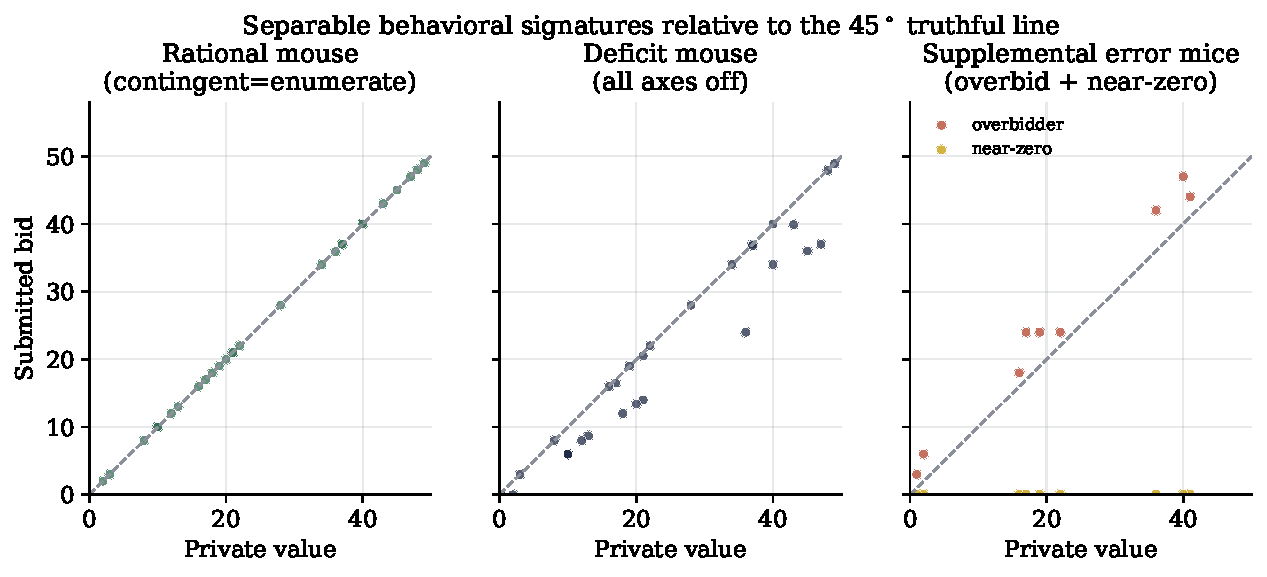
\includegraphics[width=\textwidth]{fig2.pdf}
\caption{Separable behavioral signatures. Bid versus private value for a
rational basis strain, the all-deficits-off strain, and the two supplemental
error mice. The dashed line is the $45^\circ$ truthful benchmark.}
\label{fig:signatures}
\end{figure}

\section{Result 2: Calibration Coverage}

Construct validity establishes that the axes do what theory says. Calibration
asks a different question: does the panel \emph{span} the space of mistakes that
real people make in this mechanism? We score five canonical SPSB human-mistake
classes and ask, for each, whether some strain in the panel reproduces it at a
rate above a detection threshold.

Figure~\ref{fig:coverage} and Table~\ref{tab:calibration} report the scorecard.
All five classes are covered. Truthful and overbidding behavior are reproduced
at very high rates ($0.97$ and $1.00$); moderate underbidding, extreme
overbidding, and near-zero bidding are reproduced at plausible intermediate
rates ($0.63$, $0.44$, $0.78$). The best strain for each class is reported in
the table: truthfulness and underbidding are covered by the clean procedural
basis, whereas the overbidding and near-zero classes are covered by the
targeted error mice---making explicit which classes the procedural construction
reaches on its own and which require hand-specified heuristics.

\begin{figure}[t]
\centering
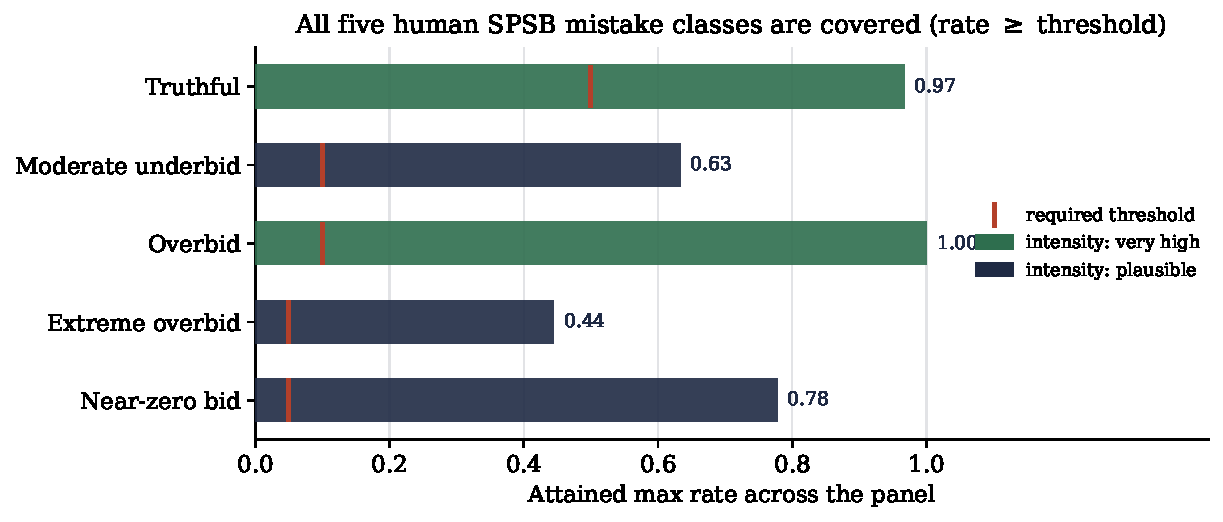
\includegraphics[width=\textwidth]{fig3.pdf}
\caption{Calibration coverage. For each human-mistake class, the maximum rate
attained by any strain in the panel (bar) against the required detection
threshold (red marker). Bar color encodes the intensity band. All five classes
clear their threshold.}
\label{fig:coverage}
\end{figure}

\begin{table}[t]
\centering
\caption{Calibration scorecard for the five canonical SPSB mistake classes.
``Max rate'' is the highest rate attained by any strain; ``best strain'' is the
strain attaining it. All classes are covered.}
\label{tab:calibration}
\footnotesize
\setlength{\tabcolsep}{3.5pt}
\begin{tabular}{@{}llrrlll@{}}
\toprule
Mistake class & Metric & \multicolumn{1}{c}{Thresh.} & \multicolumn{1}{c}{Max rate} & Best strain & Intensity & Covered \\
\midrule
Truthful         & truthful rate           & $0.50$ & $0.967$ & \texttt{c1\_f0\_b0} & very high & \checkmark \\
Moderate underbid& moderate underbid rate  & $0.10$ & $0.633$ & \texttt{c0\_f0\_b0} & plausible & \checkmark \\
Overbid          & overbid rate            & $0.10$ & $1.000$ & overgeneralizer$^\dagger$ & very high & \checkmark \\
Extreme overbid  & extreme overbid rate    & $0.05$ & $0.444$ & overgeneralizer$^\dagger$ & plausible & \checkmark \\
Near-zero bid    & near-zero bid rate      & $0.05$ & $0.778$ & payment panic$^\dagger$ & plausible & \checkmark \\
\bottomrule
\end{tabular}

\vspace{0.4em}
\begin{minipage}{0.95\textwidth}
{\footnotesize\textit{Notes.} Coverage rate $=1.00$ (5 of 5). $^\dagger$
Supplemental error strain
(\texttt{spsb\_error\_second\_price\_overgeneralizer},
\texttt{spsb\_error\_payment\_panic\_near\_zero}); all other best strains are
members of the clean $27$-cell procedural basis.\par}
\end{minipage}
\end{table}

\section{Result 3: Demonstrations Sharpen Induction}

The panel so far induces a deficit by \emph{instruction}. A natural alternative,
familiar from few-shot chain-of-thought prompting, is to also \emph{demonstrate}
the bounded procedure with a worked example. We append to a persona a single
worked example that walks through the allowed reasoning on a sample value and
ends in a bid: a margin-of-safety underbid for the all-deficit strain, and the
contingent/forward/belief reasoning that yields a truthful Vickrey bid for the
all-repaired strain. We then compare instruction-only and demonstration-augmented
personas on \emph{identical} second-price value draws.

Table~\ref{tab:cot} shows that demonstrations make induction both sharper and
more consistent. For the all-deficit strain, adding the worked example pulls the
mean bid/value ratio down toward the demonstrated $\approx 0.7$ and eliminates
truthful bidding entirely (truthful rate $0.39\to0.00$) while \emph{lowering} the
dispersion of bid/value ratios ($\operatorname{sd}0.124\to0.081$). For the
all-repaired strain, the truthful demonstration produces exact Vickrey
truth-telling on every decision (truthful rate $0.83\to1.00$, dispersion
$0.076\to0.000$). Demonstration is thus a stronger control than instruction: it
lowers behavioral variance and makes the mouse follow the prescribed procedure
more faithfully---a promising lever for the portability problem documented below,
since a more forcefully induced deficit should be harder for a capable model to
``repair'' away.

\begin{table}[t]
\centering
\caption{Instruction-only versus chain-of-thought (CoT) demonstration, on
identical second-price draws ($n=18$ bidder-decisions per cell). Demonstration
shifts behavior toward the demonstrated procedure and lowers the dispersion of
bid/value ratios.}
\label{tab:cot}
\small
\setlength{\tabcolsep}{6pt}
\begin{tabular}{@{}llrrr@{}}
\toprule
Strain & Construction & mean $b/v$ & truthful rate & $\operatorname{sd}(b/v)$ \\
\midrule
\texttt{c0\_f0\_b0} (all-deficit)  & instruction only     & $0.89$ & $0.39$ & $0.124$ \\
\texttt{c0\_f0\_b0} (all-deficit)  & + CoT demonstration  & $0.77$ & $0.00$ & $0.081$ \\
\addlinespace
\texttt{c2\_f2\_b2} (all-repaired) & instruction only     & $0.98$ & $0.83$ & $0.076$ \\
\texttt{c2\_f2\_b2} (all-repaired) & + CoT demonstration  & $1.00$ & $1.00$ & $0.000$ \\
\bottomrule
\end{tabular}
\end{table}

\section{Result 4: A First-Price Stress Test and Cross-Model Portability}

A panel is useful for screening only if it reproduces known mechanism
regularities and if its verdicts are not an artifact of the base model. We test
both. For the first, we move from the second-price environment to a
\emph{first-price} sealed-bid auction, where theory and human data are sharp:
with $n=3$ risk-neutral bidders and uniform values, the symmetric Bayes--Nash
equilibrium is to shade to $b=\frac{n-1}{n}v=\frac{2}{3}v$, and the canonical
experimental regularity is overbidding \emph{relative} to this risk-neutral
benchmark \citep{kagellevin1993}.

Figure~\ref{fig:fpsb} and Table~\ref{tab:fpsb} report the panel's first-price
behavior. The three reasoning strains track the equilibrium closely: their median
bid/value ratios are $0.65$--$0.67$, essentially on the $\frac{2}{3}$ BNE line,
and across all reasoning decisions the mean ratio is $0.67$ with $38\%$ of bids
above the risk-neutral benchmark---the documented overbidding regularity. The two
error mice separate cleanly and \emph{mechanistically}: the payment-panic mouse
bids near zero, while the second-price-overgeneralizer mouse bids \emph{above its
value} (median ratio $1.15$), because it applies the second-price intuition ``I
will not pay my own bid'' to a mechanism where the winner does pay their own bid.
In a first-price auction that error is not harmless---it yields negative
surplus---giving a concrete, mechanism-level account of a winner's-curse
pathology.

\begin{figure}[t]
\centering
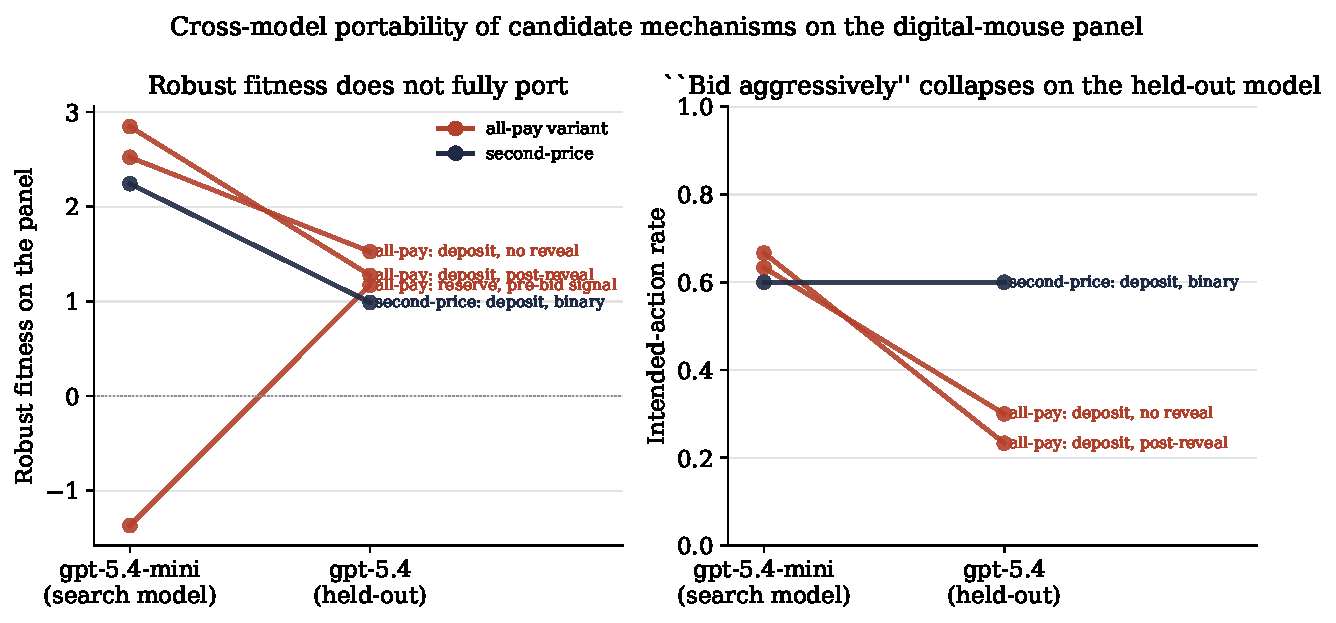
\includegraphics[width=0.82\textwidth]{fig4.pdf}
\caption{First-price stress test. Submitted bid versus private value for the
panel. Reasoning strains cluster on the risk-neutral BNE line $b=\frac{2}{3}v$;
the second-price-overgeneralizer mouse bids above the $45^\circ$ value line
(loss-making overbidding); the payment-panic mouse bids near zero.}
\label{fig:fpsb}
\end{figure}

\begin{table}[t]
\centering
\caption{First-price bid/value ratios by strain ($n=9$ bidder-decisions each).
The risk-neutral BNE benchmark is $\frac{2}{3}\approx0.667$. Reasoning strains
sit on the benchmark; the error mice separate above value and near zero.}
\label{tab:fpsb}
\small
\setlength{\tabcolsep}{6pt}
\begin{tabular}{@{}llrr@{}}
\toprule
Strain & Role & mean $b/v$ & median $b/v$ \\
\midrule
\texttt{c0\_f0\_b0} & reasoning (all-deficit) & $0.61$ & $0.65$ \\
\texttt{c2\_f0\_b2} & reasoning (forward-off) & $0.61$ & $0.67$ \\
\texttt{c2\_f2\_b2} & reasoning (all-repaired) & $0.52$ & $0.66$ \\
overgeneralizer     & error: overbid          & $1.61$ & $1.15$ \\
payment panic       & error: near-zero        & $0.02$ & $0.01$ \\
\bottomrule
\end{tabular}

\vspace{0.4em}
\begin{minipage}{0.95\textwidth}
{\footnotesize\textit{Notes.} Pooled over reasoning strains, the mean ratio is
$0.67$ (the BNE), $38\%$ of bids exceed the benchmark, and $20\%$ exceed value.
The overgeneralizer's above-value bids are loss-making under first-price
pricing.\par}
\end{minipage}
\end{table}

\paragraph{Strain-level portability.} The first-price result raises a prior
question: do the deficit \emph{strains} themselves behave consistently across
models? A pilot exposed a failure mode---the stronger model spontaneously
``repaired'' the most deficient basis strain into truthful Vickrey bidding---so
we hardened the panel into a \emph{strict} scaffold that states the
reasoning-procedure constraint explicitly rather than as a secondary goal. We
then re-ran five reserved strict strains under both base models and compared
their dominant behavioral class (Table~\ref{tab:strict}). Four of five strains
preserve their dominant class across models---a partial pass. The exception is
the strain isolating a contingent-reasoning deficit, whose moderate-underbidding
signature on \texttt{gpt-5.4-mini} is repaired into truthful bidding on
\texttt{gpt-5.4} (truthful rate $0.33\to1.00$). Consistent with the
construct-validation finding that contingent reasoning is the highest-leverage
axis (Table~\ref{tab:construct}), it is also the hardest deficit to hold fixed
against a more capable model: the strict scaffold mitigates the portability
problem but does not fully close it.

\begin{table}[t]
\centering
\caption{Strain-level cross-model portability on the strict panel. Dominant
behavioral class of five reserved strict strains under each base model. Four of
five agree; the contingent-isolated strain's deficit is repaired away by the
stronger model.}
\label{tab:strict}
\footnotesize
\setlength{\tabcolsep}{6pt}
\begin{tabular}{@{}lllc@{}}
\toprule
Strain & Isolated role & mini $\to$ gpt-5.4 (dominant class) & Agree \\
\midrule
\texttt{c2\_f2\_b0} & belief deficit          & truthful $\to$ truthful                   & \checkmark \\
\texttt{c2\_f0\_b2} & forward deficit         & mod.\ underbid $\to$ mod.\ underbid        & \checkmark \\
\texttt{c0\_f0\_b1} & near-all-defect         & mod.\ underbid $\to$ mod.\ underbid        & \checkmark \\
\texttt{c1\_f1\_b1} & all-intermediate        & truthful $\to$ truthful                   & \checkmark \\
\texttt{c0\_f2\_b2} & contingent deficit      & mod.\ underbid $\to$ \textbf{truthful}     & --- \\
\bottomrule
\end{tabular}

\vspace{0.4em}
\begin{minipage}{0.95\textwidth}
{\footnotesize\textit{Notes.} Agreement $=4/5$. ``Isolated role'' names the axis
held in its deficit state (others repaired), or a corner strain. The
contingent-deficit strain's truthful rate rises $0.33\to1.00$ across models;
all other strains' dominant class is stable.\par}
\end{minipage}
\end{table}

\section{Discussion}

\paragraph{Procedural basis versus authored error mice.} The construct-validity
result is strongest for the procedural basis, where a single instruction
(repair an axis) produces the predicted directional movement. The calibration
result is more nuanced: the basis covers truthful and underbidding behavior on
its own, but overbidding---a first-order regularity in human auction data
\citep{kagellevin1993}---is recovered only with hand-specified heuristic
strains. This distinction matters for interpretation. The model-agnostic claim
applies cleanly to the procedural axes; the error mice are a complementary,
more bespoke device for spanning the mistake space. The two should be reported
as distinct epistemic objects.

\paragraph{Model dependence.} Because deficits are defined as procedural
controls rather than artifacts of one model, the protocol can be rerun on a
different frontier model. At the strain level (Section~7), four of five reserved
strict strains preserve their dominant behavioral class across base models, the
lone exception being the contingent-reasoning deficit, which a stronger model
tends to repair into truthful bidding. This is a feature of the design rather
than a bug---the panel is precisely the instrument that makes such repair
visible---but it cautions against reading single-model panel scores as
model-invariant and identifies contingent reasoning as the deficit most in need
of a hardened scaffold. The chain-of-thought result (Section~6) suggests one
remedy: demonstration induces deficits more forcefully than instruction, and so
should be harder for a capable model to override.

\paragraph{External validity.} Digital mice are a phase-I screening population.
A strain reproducing a mistake class establishes that the panel can express that
behavior, not that the human share of that behavior is matched. We therefore
keep the stress-testing claim (this paper) separate from any calibrated
prediction of human behavior, which would require human pilot data.

\section{Conclusion}

We show that a frontier reasoning model can be instructed into stable, separable
cognitive deficits whose behavior in a second-price sealed-bid auction (i) moves
in the theory-predicted direction as each cognitive axis is repaired and (ii)
spans the canonical space of human SPSB mistakes once a small set of targeted
error strains is added, and (iii) reproduces sharp mechanism regularities in a
first-price stress test---reasoning strains shade to the risk-neutral BNE and
overbid relative to it, while an overgeneralizing strain bids above value and
loses money. We further find that worked chain-of-thought demonstrations induce
deficits more forcefully than instructions, and that most reserved deficits
preserve their behavioral class across base models. This supports a research
program in which instructed language-model agents are used as a phase-I
population to screen mechanisms for robustness to bounded rationality before
human-subject experiments are run. The immediate next steps are to extend the
cross-model and first-price analyses at scale and to carry both the
construct-validation and calibration protocols into a second domain (matching).

\begin{thebibliography}{9}
\footnotesize
\bibitem[Crawford and Iriberri(2007)]{crawfordiriberri2007}
Crawford, V.~P., and N.~Iriberri (2007). ``Level-$k$ Auctions: Can a Nonequilibrium
Model of Strategic Thinking Explain the Winner's Curse and Overbidding in
Private-Value Auctions?'' \textit{Econometrica}, 75(6), 1721--1770.

\bibitem[Eyster and Rabin(2005)]{eysterrabin2005}
Eyster, E., and M.~Rabin (2005). ``Cursed Equilibrium.''
\textit{Econometrica}, 73(5), 1623--1672.

\bibitem[Kagel and Levin(1993)]{kagellevin1993}
Kagel, J.~H., and D.~Levin (1993). ``Independent Private Value Auctions:
Bidder Behaviour in First-, Second- and Third-Price Auctions with Varying
Numbers of Bidders.'' \textit{The Economic Journal}, 103(419), 868--879.

\bibitem[Li(2017)]{li2017}
Li, S. (2017). ``Obviously Strategy-Proof Mechanisms.''
\textit{American Economic Review}, 107(11), 3257--3287.

\bibitem[Vickrey(1961)]{vickrey1961}
Vickrey, W. (1961). ``Counterspeculation, Auctions, and Competitive Sealed
Tenders.'' \textit{The Journal of Finance}, 16(1), 8--37.
\end{thebibliography}

\end{document}
